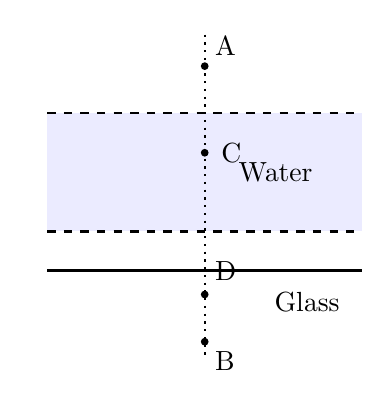
\begin{tikzpicture}[line width=0.8pt]
  % water layer (light, dashed borders)
  \fill[blue!8] (0,2.5) rectangle (4,4.0);
  \draw[dashed] (0,4.0) -- (4,4.0);
  \draw[dashed] (0,2.5) -- (4,2.5);
  \node at (2.9,3.25) {Water};
  % glass surface (solid line)
  \draw[line width=1pt] (0,2.0) -- (4,2.0);
  \node[left] at (0,3.25) {};
  \node at (3.3,1.6) {Glass};
  % vertical ray through the points
  \draw[dotted] (2,5.0) -- (2,0.9);
  % points A C D B
  \fill (2,4.6) circle (1.4pt); \node[above right] at (2,4.6) {A};
  \fill (2,3.5) circle (1.4pt); \node[right] at (2.08,3.5) {C};
  \fill (2,1.7) circle (1.4pt); \node[above right] at (2,1.75) {D};
  \fill (2,1.1) circle (1.4pt); \node[below right] at (2,1.1) {B};
\end{tikzpicture}
